\documentclass[12pt]{article}

\usepackage{amsthm}
\usepackage{graphicx}
\usepackage{float}

\newtheorem{theorem}{Theorem}[section]
\newtheorem{lemma}[theorem]{Lemma}
\newtheorem*{remark}{Remark}

\begin{document}
    \section{Model}
        $m$ machines (indexed by $i$), $n$ jobs indexed by $j$. Objective function is Total Weighted Completion time so we can suppose that the jobs are already sorted in the order $\bigg(\frac{w_j}{p_j}\bigg)_j$.\\
        Let $a_k$ be the pattern $k$. It is a binary vector of length $n$; $a_{k,j} = 1 \Leftrightarrow $ job $j$ is included in the pattern $k$.\\
        $y_{i,k}$ is the binary decision variable: $y_{i,k} = 1 \Leftrightarrow $ we use pattern $k$ for the machine $i$.
        The objective function is: 
        $$ min \sum_i \sum_k C(a_k, y_{i,k}) $$ 
        with $C(a_k, y_{i,k}) = y_{i,k} \sum_j a_{k,j} w_j \sum_s^j a_{k,j} p_j^i $ 

        This formulation of $C$ can be justified by analogy to the following programs (that are equivalent):

        \begin{figure}[H]
            \centering
            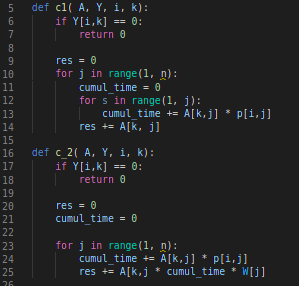
\includegraphics[scale = 0.8]{p3_c1_c2.png}
        \end{figure}

        Constraints are:
        $$ \forall i, \sum_k y_{i,k} = 1   $$
        $$ \forall j, \sum_{i, k} a_{k, j} y_{i,k} = 1  $$

    \section{Reduced cost}
        Let $u_i$, $v_j$ be the dual variables.
        The reduced cost is:

        $$ $$

\end{document}